\documentclass[crop,tikz]{standalone}

\tikzset{>=latex}
\usetikzlibrary{calc}

\begin{document}
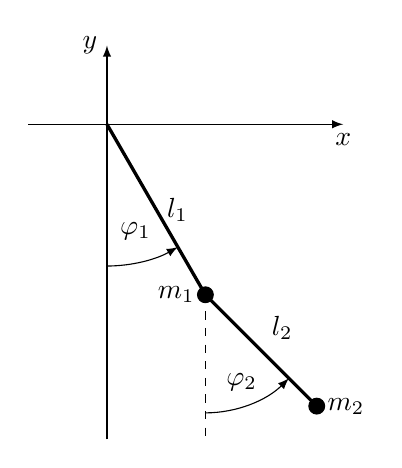
\begin{tikzpicture}
  \pgfmathsetmacro{\phiA}{30};
  \pgfmathsetmacro{\phiB}{45};
  \pgfmathsetmacro{\lenA}{2.5};
  \pgfmathsetmacro{\lenB}{2};
  \draw[->] (-1,0) -- (3,0) node[below] {$x$};
  \draw[->] (0,-4) -- (0,1) node[left] {$y$};
  \draw[fill] ({-90+\phiA}:\lenA) circle (0.1) coordinate (P);
  \draw[fill] (P)++(-\phiB:\lenB) circle (0.1) coordinate (Q);
  \draw[very thick] (0,0) -- node[right] {$l_1$} (P) node[left] {$m_1$} -- node[above right] {$l_2$} (Q) node[right] {$m_2$};
  \draw[dashed] (P) -- ++(0,{-4+\lenA*cos(\phiA)});
  \draw[->] (0,-1.8) arc (-90:{-90+\phiA}:1.8);
  \node at ({-90+\phiA/2}:1.4) {$\varphi_1$};
  \draw[->] (P)++(0,-1.5) arc (-90:{-90+\phiB}:1.5);
  \node at ($(P)+({-90+\phiB/2}:1.2)$) {$\varphi_2$};
\end{tikzpicture}
\end{document}
